\documentclass[a4paper,12pt]{article}
\usepackage{fancyhdr}
\usepackage{fancyheadings}
\usepackage[ngerman,german]{babel}
\usepackage{german}
\usepackage[utf8]{inputenc}
%\usepackage[latin1]{inputenc}
\usepackage[active]{srcltx}
\usepackage{algorithm}
\usepackage[noend]{algorithmic}
\usepackage{amsmath}
\usepackage{amssymb}
\usepackage{amsthm}
\usepackage{bbm}
\usepackage{enumerate}
\usepackage{graphicx}
\usepackage{ifthen}
\usepackage{listings}
\usepackage{struktex}
\usepackage{hyperref}

% Führende Null mitziehen
\newcommand{\leadingzero}[1]{\ifnum #1<10 0\the#1\else\the#1\fi}
\renewcommand{\today}{\leadingzero{\day}.\leadingzero{\month}.\the\year}     % DD.MM.YYYY
 
 % Anfuehrungszeichen
\newcommand{\An}[1]{\glqq #1\grqq{}} 
 	

%%%%%%%%%%%%%%%%%%%%%%%%%%%%%%%%%%%%%%%%%%%%%%%%%%%%%%
%%%%%%%%%%%%%% EDIT THIS PART %%%%%%%%%%%%%%%%%%%%%%%%
%%%%%%%%%%%%%%%%%%%%%%%%%%%%%%%%%%%%%%%%%%%%%%%%%%%%%%
\newcommand{\Fach}{Brückenkurs Mathe}
\newcommand{\Modulnummer}{09804}
\newcommand{\Name}{Jonathan Skopp}
\newcommand{\Datum}{\today}
\newcommand{\Matrikelnummer}{3301729}
\newcommand{\Semester}{WS 20/21}
\newcommand{\Uebungsblatt}{1}
%%%%%%%%%%%%%%%%%%%%%%%%%%%%%%%%%%%%%%%%%%%%%%%%%%%%%%
%%%%%%%%%%%%%%%%%%%%%%%%%%%%%%%%%%%%%%%%%%%%%%%%%%%%%%



\setlength{\parindent}{0em}
\topmargin -1.0cm
\oddsidemargin 0cm
\evensidemargin 0cm
\setlength{\textheight}{9.2in}
\setlength{\textwidth}{6.0in}


\newcommand{\Aufgabe}[1]{
  {
  \vspace*{0.5cm}
  \textsf{\textbf{Aufgabe #1}}
  \vspace*{0.2cm}
  
  }
}
%%%%%%%%%%%%%%
\hypersetup{
    pdftitle={\Fach{}: Einsendeaufgaben \Uebungsblatt{}},
    pdfauthor={\Name},
    pdfborder={0 0 0}
}


\title{Kurseinheit  \Uebungsblatt{}}
\author{\Name{}}

\begin{document}
\thispagestyle{fancy}
\lhead{\sf \large \Fach{} - \Modulnummer \\ \small \Name{} - \Matrikelnummer{}}
\rhead{\sf \Semester{} \\  Datum \today }
\vspace*{0.2cm}
\begin{center}
\LARGE \sf \textbf{Einsendeaufgaben Kurseinheit \Uebungsblatt{}}
\end{center}
\vspace*{0.2cm}

%%%%%%%%%%%%%%%%%%%%%%%%%%%%%%%%%%%%%%%%%%%%%%%%%%%%%%
%% Insert your solutions here %%%%%%%%%%%%%%%%%%%%%%%%
%%%%%%%%%%%%%%%%%%%%%%%%%%%%%%%%%%%%%%%%%%%%%%%%%%%%%%

\Aufgabe{1}
Gegeben seien die beiden Aussagen: 
\begin{itemize}
	\item[A: ] Das Ziel ist erreicht.
	\item[B: ] Alle Bedingungen sind erfüllt.
\end{itemize}

Übersetzen Sie die folgenden zusammengesetzten Aussagen in die Symbolsprache:\\

Es gilt weiterhin: 
\begin{eqnarray}
	(A \lor \lnot A) \equiv \text{\An{wahr}}\\
	(A \land \lnot A) \equiv \text{\An{falsch}}
\end{eqnarray}
Dabei sind $A$ und $B$ austauschbar.


\begin{itemize}
	\item[a)] 	
		Das Ziel ist erreicht und alle Bedingungen sind erfüllt.\\

Es ist zu erkennen, das $A$ und $B$ immer wahr sein sollen.

\begin{eqnarray}
\Sigma_{a} = \left( A \lor \lnot A \right) \land   \left( B \lor \lnot B \right)
\end{eqnarray}
Die Tautologien eliminiert alle Belegungen in denen $A$ oder $B$ falsch ist. Dadurch kann garantiert werden, dass sowohl $A$ und $B$ wahr sind. 

	 \item[b)]
	 	Das Ziel ist erreicht, obwohl nicht alle Bedingungen erfüllt sind.\\

$A$ soll wahr sein und $B$ darf nur falsch annehmen.

\begin{eqnarray}
\Sigma_{b} = (A \lor \lnot A) \land  (B \lor \lnot B) 
\end{eqnarray}


	 \item[c)]
	 	Weder ist das Ziel erreicht, noch sind alle Bedingungen erfüllt. \\


Es gilt, dass $A$ und $B$ nur falsch sind.

\begin{eqnarray}
	\Sigma_{c} = \left( A \land \lnot A \right) \land \left( B \land \lnot B \right)
\end{eqnarray}

Um hier eine Tautologie zu erreichen muss für $A$ und $B$ eine Kontradiktion vorliegen.
	 \item[d)] 
	 	Wenn alle Bedingungen erfüllt sind, ist das Ziel erreicht.

Hier ist $A$ von $B$ abhängig. 

\begin{eqnarray}
	\Sigma_{d} = \left( A \land \lnot A  \right) \rightarrow \left( A \right) 
\end{eqnarray}

	 \item[e)] 
	 	Wenn das Ziel erreicht ist, ist es egal, ob alle Bedingungen erfüllt sind oder nicht.

Hier geht es nur darum zu zeigen das $A \forall B$ wahr ist.

\begin{eqnarray}
	\Sigma_{e} = \left(A \lor \lnot A \right) \lor B
\end{eqnarray}
\end{itemize}
\clearpage

\Aufgabe{2}
$
	\lnot ( \lnot A \land \lnot C ) \lor ( A \land (\lnot B \lor A)) \text{~ und ~} A \lor C
$\\
\vspace{2cm}
\\
Es gilt zu zeigen, dass gilt: \\
$\lnot ( \lnot A \land \lnot C ) \lor ( A \land (\lnot B \lor A)) \equiv A \lor C$\\

Für $\lnot ( \lnot A \land \lnot C ) \lor ( A \land (\lnot B \lor A)) $:\\
\begin{center}
\begin{tabular}[h]{c|c|c|c}
 $A$ & $B$ & $C$ &  $\lnot ( \lnot A \land \lnot C ) \lor ( A \land (\lnot B \lor A))$ \\ 
 \hline
 1 & 1 & 1 & (~~1~~~0~~~0~~~0~~~*1~~~1~~0~~~1~~)\\
 1 & 1 & 0 & (~~1~~~0~~~0~~~1~~~*1~~~1~~~0~~~1~~)\\
 1 & 0 & 1 & (~~1~~~0~~~0~~~0~~~*1~~~1~~~1~~~1~~)\\
 1 & 0 & 0 & (~~1~~~0~~~0~~~1~~~*1~~~1~~~1~~~1~~)\\
 0 & 1 & 1 & (~~1~~~1~~~0~~~0~~~*1~~~0~~~0~~~0~~)\\
 0 & 1 & 0 & (~~0~~~1~~~1~~~1~~~*0~~~0~~~0~~~0~~)\\
 0 & 0 & 1 & (~~1~~~1~~~0~~~0~~~*1~~~0~~~1~~~1~~)\\
 0 & 0 & 0 & (~~0~~~1~~~1~~~1~~~*0~~~0~~~1~~~1~~)\\

\end{tabular}
\end{center}
\vspace{2cm}

Für $A \lor C$
\begin{center}
	\begin{tabular}[h]{c|c|c|c}
		$A$ & $B$ &  $C$ & $A \lor C$ \\ 
		\hline
		1 & 1 & 1 & 1\\
		1 & 1 & 0 & 1\\
		1 & 0 & 1 & 1\\
		1 & 0 & 0 & 1\\
		0 & 1 & 1 & 1\\
		0 & 1 & 0 & 0\\
		0 & 0 & 1 & 1\\
		0 & 0 & 0 & 0\\
	\end{tabular}
\end{center}

\vspace{1cm}
$ \left(1,1,1,1,1,1,0,1,0\right) \equiv \left(1,1,1,1,1,1,0,1,0\right) $\\
Die Aussagen sind äquivalent.
\clearpage

\Aufgabe{3}
\begin{eqnarray}
	M_1 \cup M_2 = \left\{ 1,2,3,4,5,6,7 \right\}\\
	M_2 \cap M_1 = \left\{ 1,3,5,7       \right\}\\
	M_1 \setminus M_2 = \left\{ 2,4,6 \right\} \\
	M_2 \setminus M_1 = \varnothing
\end{eqnarray}
Gesucht sind die Mengen $M_1$ und $M_2$.\\ \vspace{2cm}
\\
Wir nehmen an, dass alle Elemente in $\mathbb{N}$ liegen:\\
\begin{eqnarray}
	M_1 = \{x \in \mathbb{N} | x \in M_1 \}\\
	M_2 = \{x \in \mathbb{N} | x \in M_2 \}
\end{eqnarray}
Aus der Vereinigung können wir Rückschlüsse auf die Grundmenge ziehen: \\

\begin{eqnarray}
	M_1 \cup M_2 = \Omega = \left\{ 1,2,3,4,5,6,7 \right\}
\end{eqnarray}

Wenn man nun die Differenz der beiden Mengen betrachtet wird deutlich, dass $M_1$ eine größere Kardinalität aufweist als $M_2$:
\begin{eqnarray}
	\vert M_1 \setminus M_2 \vert > \vert M_2 \setminus M_1 \vert\\
	\vert \{2,4,6\} \vert > \vert \varnothing \vert \\
	3 > 0
\end{eqnarray}
Dadurch sehen wir, dass es mehr Elemente in $M_1$ gibt als in $M_2$. \\
Um weitere Rückschlüsse auf $M_1$ und $M_2$ zu bekommen, ziehen wir die Schnittmenge der beiden heran. 
\begin{eqnarray}
	M_1 \cap M_2 = \left\{x \in \mathbb{N} \vert x \in M_1 \land x \in M_2 \right\}
\end{eqnarray}
Daraus kann nun $M_1$ abgeleitet werden.: 
\begin{eqnarray}
	M_1 = (M_1 \cap M_2) \cup  ( M_1 \setminus M_2) \\
	M_1 = \left\{ 1,3,5,7 \right\} \cup \left\{ 2,4,6 \right\}\\
	M_1 = \left\{ 1,2,3,4,5,6,7 \right\}
\end{eqnarray}
Da nun $M_1$ bekannt ist, können wir auch $M_2$ ermitteln.
\begin{eqnarray}
	M_2 \cap M_1 = \left\{ 1,3,5,7       \right\}\\
	M_2 = \left\{ 1,3,5,7       \right\}
\end{eqnarray}
Diese Aussage ist wahr, da $M_1$ als $\Omega$ (Grundmenge) angesehen werden kann.



\clearpage


\Aufgabe{4}
Es gibt 3 Maschinen. Diese werden im folgenden $A$,$B$,$C$ genannt. \\
Ferner gibt es 8 Produkte die wie folgt auf den Maschinen abgebildet werden.

\begin{eqnarray}
	\Omega = \left\{a_1, a_2,\cdots,a_8\right\}\\
	A = \left\{  a_1, a_2,a_3,a_4,a_5\right\}\\
	B = \left\{a_1,a_3,a_4,a_6, a_7\right\}\\
	C = \left\{ a_1, a_4, a_6, a_7, a_8 \right\}
\end{eqnarray}\\

\begin{itemize}
	\item[i)] 	
	auf allen drei Maschinen bearbeitet werden.

\begin{align}
	 A \cap B \cap C\\
	& =\left\{  a_1, a_2,a_3,a_4,a_5\right\} \cap \left\{a_1,a_3,a_4,a_6, a_7\right\} \cap \left\{ a_1, a_4, a_6, a_7, a_8 \right\}\\
	& = \left\{a_1,a_4\right\} 
\end{align}
	\item[ii)]
	nur auf der Maschine $A$ bearbeitet werden.
\begin{align}
	 A \setminus B \setminus C \\
	 	& =\left\{  a_1, a_2,a_3,a_4,a_5\right\} \setminus \left\{a_1,a_3,a_4,a_6, a_7\right\} \setminus \left\{ a_1, a_4, a_6, a_7, a_8 \right\}\\
	& = \left\{a_2,a_5\right\}
\end{align}
	\item[iii)]
	nur auf Maschine B bearbeitet werden

\begin{align}
	 B \setminus C \setminus A \\
	& = \left\{a_1,a_3,a_4,a_6, a_7\right\} \setminus  \left\{ a_1, a_4, a_6, a_7, a_8 \right\} \setminus \left\{  a_1, a_2,a_3,a_4,a_5\right\}\\
	& = \emptyset
\end{align}
	\item[iv)] 
	nur auf der Maschine C bearbeitet werden.

\begin{align}
	 C \setminus B \setminus A \\
	& = \left\{ a_1, a_4, a_6, a_7, a_8 \right\} \setminus \left\{a_1,a_3,a_4,a_6, a_7\right\} \setminus \left\{  a_1, a_2,a_3,a_4,a_5\right\} \\
	& = \left\{a_8\right\}
\end{align}
	\item[v)] 
	auf der Maschine A oder C bearbeitet werden.

\begin{align}
	 A \cup C\\
	&= \left\{  a_1, a_2,a_3,a_4,a_5\right\} \cup  \left\{ a_1, a_4, a_6, a_7, a_8 \right\} \\
	& = \Omega \\
	&=\left\{a_1, a_2,\cdots,a_8\right\}
\end{align}
	\item[vi)] 
	auf der Maschine B oder C  bearbeitet werden.

\begin{align}
	 \left\{x \in \Omega \vert x\in B \land x\in C\right\}\\
	 &= \left\{a_1,a_3,a_4,a_6, a_7\right\} \cup \left\{ a_1, a_4, a_6, a_7, a_8 \right\}\\
	& = \left\{a_1, a_3, a_4,a_6,a_7,a_8\right\} 
\end{align}
\end{itemize}
\clearpage

\Aufgabe{5}
Gegeben seien die Mengen: 

\begin{eqnarray}
	A = \left\{ \left(x,y \right) \in \mathbb{R} \times \mathbb{R}: x^2 +y^2 \le 16 \right\}\\
	B = \left\{ \left(x,y \right) \in \mathbb{R_{+}} \times \mathbb{R_{+}}: x > \sqrt{y} \right\}\\
	C = \left\{ \left(x,y \right) \in \mathbb{R} \times \mathbb{R}: y > -\dfrac{1}{2}x+3 \right\}\\
	D = \left\{ \left(x,y \right) \in \mathbb{R} \times \mathbb{R}: y \ge x^2 \right\}
\end{eqnarray}
Die Ermittlung der Hilfspunkte sind in Aufgabe 5b zu finden.\\
\begin{itemize}
	\item[a)] 	
	Skizzieren Sie alle Mengen in einem Koordinatensystem, und kennzeichnen 
Sie darin die Menge 

\begin{eqnarray}
	\Sigma = A \cap B \cap C \cap D
\end{eqnarray}

	\begin{figure}[h]
		\centering
		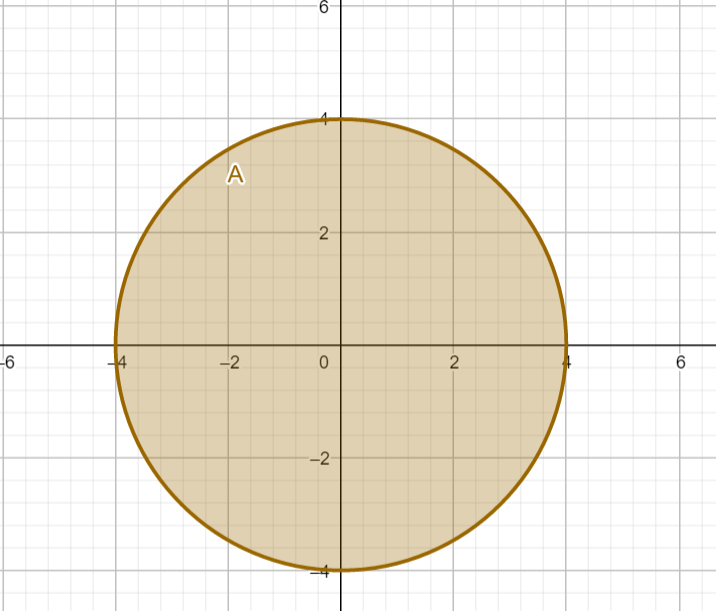
\includegraphics[width=6cm,height=4cm]{MengeA.png}
		\caption{$A = \left\{ \left(x,y \right) \in \mathbb{R} \times \mathbb{R}: x^2 +y^2 \le 16 \right\}$}
		\label{fig:Menge A}
	\end{figure}

	\begin{figure}[h]
	\centering
	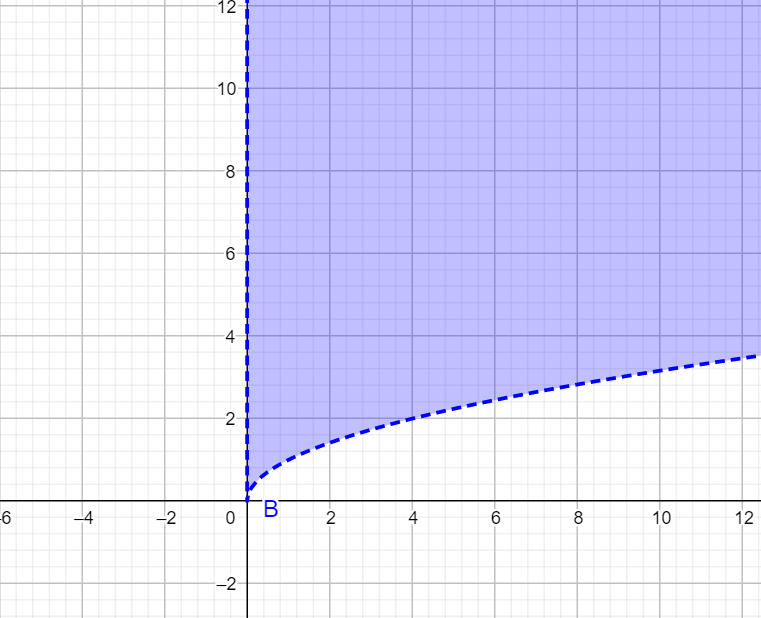
\includegraphics[width=6cm,height=4cm]{MengeB.png}
	\caption{$B=\left\{ \left(x,y \right) \in \mathbb{R_{+}} \times \mathbb{R_{+}}: x > \sqrt{y} \right\}$}
	\label{fig:Menge B}
\end{figure}

\begin{figure}[h]
	\centering
	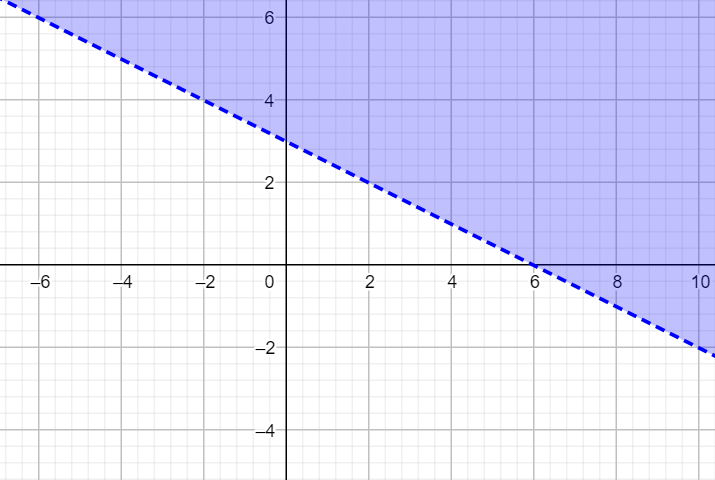
\includegraphics[width=6cm,height=4cm]{MengeC.png}
	\caption{$C = \left\{ \left(x,y \right) \in \mathbb{R} \times \mathbb{R}: y > -\dfrac{1}{2}x+3 \right\}$}
	\label{fig:Menge C}
\end{figure}

\begin{figure}[h]
	\centering
	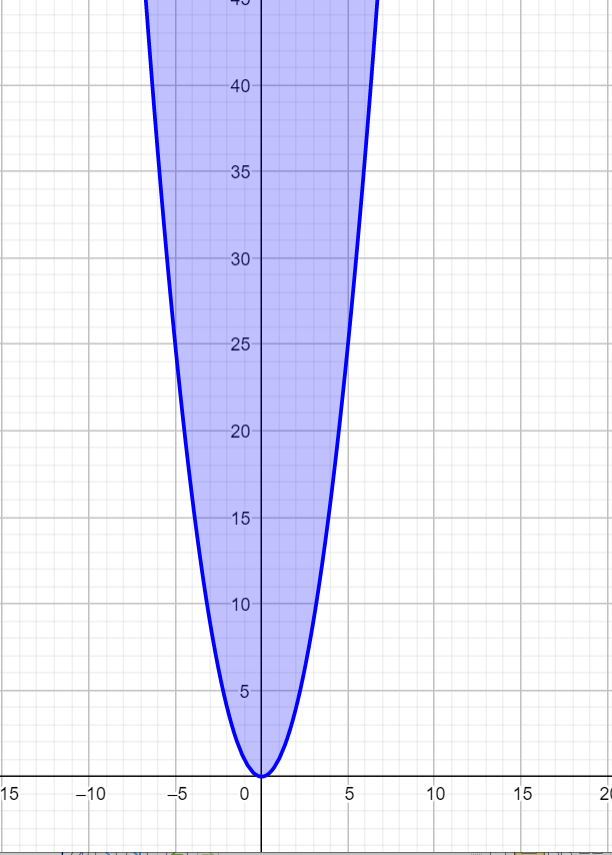
\includegraphics[width=6cm,height=4cm]{MengeD.png}
	\caption{$D = \left\{ \left(x,y \right) \in \mathbb{R} \times \mathbb{R}: y \ge x^2 \right\}$}
	\label{fig:Menge D}
\end{figure}

\begin{figure}[h]
	\centering
	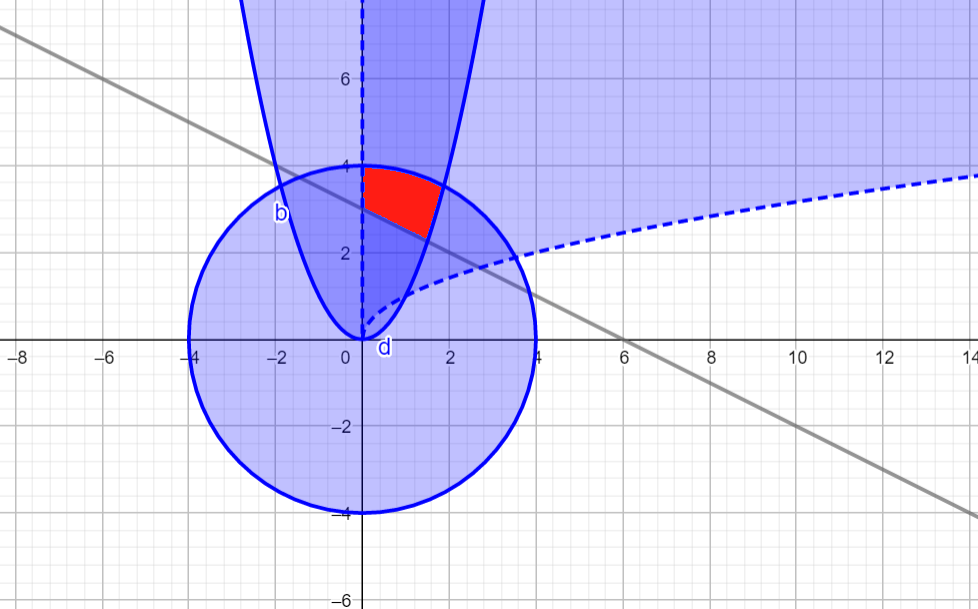
\includegraphics[width=6cm,height=4cm]{MengeE.png}
	\caption{$\Sigma = A \cap B \cap C \cap D$}
	\label{fig:Menge D}
\end{figure}
\clearpage
	\item[b)]
	Bestimmen Sie die Menge: 
\begin{eqnarray}
	\left(A \cap B \cap C \cap D \right) \times \left(\mathbb{N}_0 \times \mathbb{N}_0 \right)
\end{eqnarray}

Lösung + Punkte aus 5a: \\


Definition $\mathbb{N}_0$:
\begin{eqnarray}
	N_0 = \left\{x \in \mathbb{Z} \vert x \ge 0 \right\}
\end{eqnarray}

Allgemein gilt daher:
\begin{eqnarray}
	\left(A \cap B \cap C \cap D \right)  = E \vert  \text{~~~aus a~}\\
	\left(A \cap B \cap C \cap D \right) \times \left(N_0 \times N_0 \right)\\
	E \times (\{x\in \mathbb{Z}\vert x \ge 0\}\times \{x\in \mathbb{Z}\vert x \ge 0\}) 
\end{eqnarray}

Betrachten wir nun $A$ im Zahlenbereich $\mathbb{N}_0$ fallen uns folgende Tupel auf: \\
\begin{eqnarray}
	\left\{ (-4,0);(0,4); (0,-4); (4,0)\right\}\in A_{\mathbb{N}_0} 
\end{eqnarray}

Betrachten wir nun $B$ im Zahlenbereich $\mathbb{N}_0$ fällt auf, dass der Bereich der Menge durch die positive Y-Achse und durch den Term $\sqrt(x)$ nach unten beschränkt ist. \\

Betrachten wir nun $C$ im Zahlenbereich $\mathbb{N}_0$ fällt auf, dass der Bereich der Menge durch die positive Y-Achse und durch den Term $-\dfrac{1}{2}x+3$ nach unten beschränkt ist. \\

Betrachten wir nun $D$ im Zahlenbereich $\mathbb{N}_0$ fällt auf, dass der Bereich der Menge durch die positive Y-Achse und durch den Term $x^2$ nach unten beschränkt ist.\\

Man kann dies Sich die gesuchte Flächte recht solide im Kopf vorstellen. $A$ stellt die Grundfläche ($\Omega$) dar. Diese wird dann durch die Mengen $A \cdots D$ begrenzt. So begrenzt $C$ von oben und $B$ und $D$ \An{rechts }und \An{links} \\

Die Abgeschlossene Menge hat folglich folgende Punkte in $N_0$:\\ 

\begin{eqnarray}
	E= \left\{ (1,3); (0,4) \right\} 
\end{eqnarray}

\clearpage

Für $(1,3)$ aus $\left(\mathbb{N}_0 \times \mathbb{N}_0\right)$:
\begin{itemize}
	\item A: $ x^2 +y^2 \rightarrow 1^2 + 3^2 \le 16$
	\item B: $ y > \sqrt{x} \rightarrow 3 > \sqrt{1}$
	\item C: $y > -\dfrac{1}{2}\cdot x+3 \rightarrow 3 > -\dfrac{1}{2} \cdot 1 +3 \rightarrow 3 > 2.5$
	\item D: $y \ge x^2 \rightarrow 3 \ge 1^2$
\end{itemize}
$\square$

\vspace{2cm}
Für $(0,4)$ aus $\left(\mathbb{N}_0 \times \mathbb{N}_0\right)$:
\begin{itemize}
	\item 
	A: $ x^2 +y^2 \rightarrow 0^2 + 4^2 \le 16$
	\item 
	B: $ y > \sqrt{x} \rightarrow 4 > \sqrt{0}$
	\item 
	C: $y > -\dfrac{1}{2}\cdot x+3 \rightarrow 4 > -\dfrac{1}{2} \cdot 0 +3 \rightarrow 4 > 3$
	\item
	D: $y \ge x^2 \rightarrow 4 \ge 0^2 $ 
\end{itemize}
$\square$
\end{itemize}
\clearpage


\Aufgabe{6}
Prüfen Sie die Menge auf Intervalle und notieren Sie diese gemäß Definition in Intervallschreibweise. \\

$
\begin{array}{c|c|c}
	\text{Intervallart} & \text{Definition} & \text{Beschreibung}\\
	\hline
	\left( a,b\right) & \left\{x \vert x\in \mathbb{R } \land a < x < b\right\} & \text{offenes Intervall} \\
	\left(a,b \right]  & \left\{x \vert x\in \mathbb{R } \land a < x \le b\right\} 	 & \text{halboffenes Intervall} \\
	\left[a,b \right)  & \left\{x \vert x\in \mathbb{R } \land a \le x < b\right\} 	 & \text{halboffenes Intervall} \\	
	\left[a,b \right]  & \left\{x \vert x\in \mathbb{R } \land a \le x \le b\right\} 	 & \text{geschlossenes Intervall} \\	
\end{array}
$\\
\begin{itemize}
	\item[a)] 	
	
\begin{eqnarray}
\left\{x \vert x \in \mathbb{R} \land x \le 12 \right\} \cap \left\{ x \vert x \in \mathbb{R}  \land x > 5\right\} 
\end{eqnarray}

Hierbei handelt es sich um ein Intervall.

\begin{eqnarray}
	\left\{x \in \mathbb{R} \vert x \le 12 \right\} \cap \left\{ x \in \mathbb{R}  \vert x > 5\right\} = \left(5,12\right]\\
	\left(5,12\right] =	\left\{ x \in \mathbb{R} \vert 5 < x \le 12\right\}
\end{eqnarray}

$\curvearrowright$ Es handelt sich um ein halboffenes Intervall.

$\square$
	\item[b)]
	\begin{eqnarray}
	\left\{x \vert x \in \mathbb{R}_{+} \land x < 7 \right\} \setminus \left\{ x \vert x \in \mathbb{R}  \land x \ge 5\right\} 
\end{eqnarray}
Es handelt sich um ein Intervall:\\

Anmerkung:\\
\begin{eqnarray}
	 \mathbb{R}_{+} = \left\{x \vert x \in \mathbb{R} \land x  \ge 0 \right\}
\end{eqnarray}


Deswegen gilt: \\

\begin{eqnarray}
	\left\{x \vert x \in \mathbb{R}_{+} \land x < 7 \right\} \setminus \left\{ x \vert x \in \mathbb{R}  \land x \ge 5\right\} =  \left(0,5 \right)
\end{eqnarray}
$\curvearrowright$ Es handelt sich um ein offenes Intervall.\\

\begin{eqnarray}
\left(0,5 \right) = \left\{ x | x \in \mathbb{R}_{+} \land 0<x<5 \right\}
\end{eqnarray}

$\square$
	\item[c)] 
	\begin{eqnarray}
	\left\{x \vert x \in \mathbb{R} \land -7 < x \le 3 \right\} \cap \left\{x \vert x \in \mathbb{R} \land -2 \le x < 4 \right\}
\end{eqnarray}

Hierbei handelt es sich um ein Intervall: \\

\begin{eqnarray}
	\left\{x \vert x \in \mathbb{R} \land -7 < x \le 3 \right\} \cap \left\{x \vert x \in \mathbb{R} \land -2 \le x < 4 \right\} = \left[-2,3\right]\\
	\left\{ x | x \in \mathbb{R}_{+} \land -2\le x \le 3 \right\} = \left[-2,3\right]
\end{eqnarray}
$\curvearrowright$ Es handelt sich um ein geschlossenes Intervall.


$\square$
	\item[d)]
	\begin{eqnarray}
	\left\{ x \vert x \in \mathbb{N} \land x \ge 4 \right\} \cap \left\{ x \vert x \in \mathbb{R} \land x \le 4\right\} \\
		\left\{ x \vert x \in \mathbb{N} \land x \ge 4 \right\} \cap \left\{ x \vert x \in \mathbb{R} \land x \le 4\right\} = \left\{4\right\}
\end{eqnarray}
$\curvearrowright$ Es handelt sich um kein Intervall da: \\ $\vert \left\{ x \vert x \in \mathbb{N} \land x \ge 4 \right\} \cap \left\{ x \vert x \in \mathbb{R} \land x \le 4\right\} \vert =1 $ \\
$\square$
\end{itemize}





%%%%%%%%%%%%%%%%%%%%%%%%%%%%%%%%%%%%%%%%%%%%%%%%%%%%%%
\end{document}
